\documentclass[10pt]{armath}
\usepackage{amsmath}
\usepackage{csquotes}
\usepackage{enumitem}
\usepackage{tikz}
% \usepackage[margin=1in]{geometry}

\title{Ancient Sculpture Polychromy}
\author{Arden Rasmussen}
\date{\today}

\begin{document}
\maketitle

Most sculpture that we have from ancient Greece lacks any sign of colors or
pigments. Because of this fact, the casual observer may not even consider that
this was not the intended state. However, though scientific research and
analysis of the sculptures, and through cross referencing with literary
material, we know that this is not the case. Through research we know that
practically all sculpture and architecture was brightly colored. We examine
some of the scientific methods that are utilized in order to ascertain more
insight into the original coloring of a sculpture. This is becomes very useful
when most of the pigments would have faded away due to exposure to light.

The first evidence that we have that ancient sculpture had coloring of any
form, was from the sculptures that were covered in ash in Pompeii. The ash was
able to protect the pigments from the harmful effects of sunlight. Because of
this the pigments of these sculptures were preserved significantly better than
any those used on previously discovered sculptures. This makes it clear that
the sunlight is a significantly harmful factor when it comes to pigment
preservation.

Many of the early attempts at the prediction of the colorization of the
sculpture and architecture, was done before many of the scientific techniques
that are now used today were known. This means that most of those
reconstructions were primarily based on the antithetical preferences of the
historian attempting the reconstruction. These reconstructions only accounted
for a few bits of evidence that was available at the time. The primary evidence
was if color was clearly visible on the sculpture, it if was not, then it was
up to the historian to decide what color should be placed there.

As more methods scientific methods of determining the colorization or the
pigment of sculptures were developed, the accuracy of the reconstructions began
to converge to the ground truth of how it may have been originally painted. We
will go though all of the methods that are used commonly now in order to assist
in the determination of the color if not the pigments for ancient sculpture.

\textbf{Raking Light} This is a method that involves shining light from a very
sharp angle, almost parallel to the surface of the sculpture. This method
is used to pick up on the radiation resistance of different pigments, and
colors. Anything exposed to solar radiation will get damaged over time,
some materials will get damaged faster than others. Having a paint over the
marble, acts like a shield, protecting from the solar radiation. So instead
of the marble getting damaged, the paint gets damaged instead. This means
that there will be a raised portion, where the paint was weathered away
instead of the marble. This is depicted in figure \ref{fig:raking_light_1}.

\begin{figure}[htpb]
  \begin{center}
  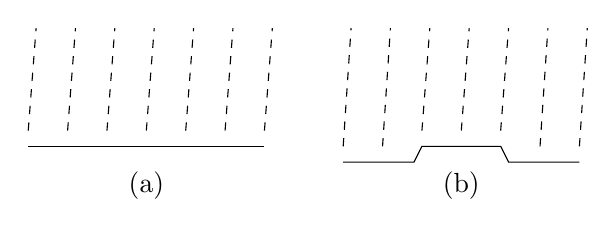
\begin{tikzpicture}[scale=1, transform shape]
    \begin{scope}[shift={(0,0)}]
      \draw (0,0) -- (1,0) -- (2,0) -- (3,0);
      \draw[dashed] (0,0.2) -- (0.1,1.5);
      \draw[dashed] (0.5,0.2) -- (0.6,1.5);
      \draw[dashed] (1,0.2) -- (1.1,1.5);
      \draw[dashed] (1.5,0.2) -- (1.6,1.5);
      \draw[dashed] (2,0.2) -- (2.1,1.5);
      \draw[dashed] (2.5,0.2) -- (2.6,1.5);
      \draw[dashed] (3,0.2) -- (3.1,1.5);
      \node (a) at (1.5, -0.5) {(a)};
    \end{scope}

    \begin{scope}[shift={(4,0)}]
      \draw (0,-0.2) -- (0.9,-0.2) -- (1,0) -- (2,0) -- (2.1,-0.2) -- (3,-0.2);
      \draw[dashed] (0,0) -- (0.1,1.5);
      \draw[dashed] (0.5,0) -- (0.6,1.5);
      \draw[dashed] (1,0.2) -- (1.1,1.5);
      \draw[dashed] (1.5,0.2) -- (1.6,1.5);
      \draw[dashed] (2,0.2) -- (2.1,1.5);
      \draw[dashed] (2.5,0) -- (2.6,1.5);
      \draw[dashed] (3,0) -- (3.1,1.5);
      \node (b) at (1.5, -0.5) {(b)};
    \end{scope}
  \end{tikzpicture}
  \end{center}
  \caption{Demonstrating the process of solar radiation wearing through the
  marble surface, where the center segment is protected by some pigment. Over
  time smooth surfaces of (a) will develop bumps like the surface of (b).}
  \label{fig:raking_light_1}
\end{figure}

This method becomes very useful to determine where different pigments were on a
sculpture, and to ascertain the location of the transitions between them. Since
each pigment would protect the underlying medium different amounts, each
pigment would leave a different sized "bump" on the sculpture. There is little
to gain about the actual color using this method, but it does allow for knowing
where the different colors start and end.

By shining a light almost perpendicular to the surface of the sculpture it is
possible to see these microscopic ridges on the surface of the sculpture. This
process is clearly depicted in \ref{fig:raking_light_2}.

\begin{figure}[htpb]
\begin{center}
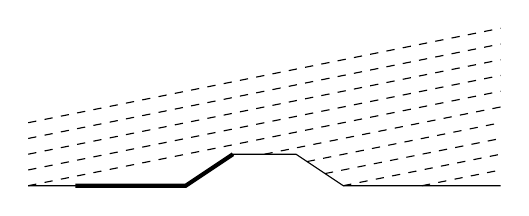
\begin{tikzpicture}[scale=2, transform shape]
  \draw (0,0) -- (1,0) -- (1.3,0.2) -- (1.7,0.2)--(2,0)--(3,0);
  \draw[line width=1.5pt] (0.3,0) -- (1,0) -- (1.3,0.2);
  \draw[dashed] (0.0,0.4) -- (3.0,1.0);
  \draw[dashed] (0.0,0.3) -- (3.0,0.9);
  \draw[dashed] (0.0,0.2) -- (3.0,0.8);
  \draw[dashed] (0.0,0.1) -- (3.0,0.7);
  \draw[dashed] (0.0,0) -- (3.0,0.6);
  \draw[dashed] (1.5,0.2) -- (3.0,0.5);
  \draw[dashed] (1.769,0.153) -- (3.0,0.4);
  \draw[dashed] (1.884,0.077) -- (3.0,0.3);
  \draw[dashed] (2.0,0) -- (3.0,0.2);
  \draw[dashed] (2.5,0) -- (3.0,0.1);
\end{tikzpicture}
\end{center}
\caption{Demonstrating how using raking light will cast shadows caused by small
ridges on the surface of a material. This allows for the determination of where
pigments would have been present.}
\label{fig:raking_light_2}
\end{figure}

This method of raking light does not provide researchers will too much
information about what pigments were actually present on a sculpture, but it
does help in the determination of the regions of different pigments. Thus if a
pigment is determined anywhere in the region, it is reasonable to  believe
that that pigment was used for the entirety of the region.

\end{document}
